\chapter{Movimiento Rectilíneo:}

\textit{``Al principio vienen necesariamente a la mente la fantasía y la fábula. Desfilan después los cálculos matemáticos, y 
solo 
al final la realización corona el pensamiento.''} \textbf{Konstantin Tsiolkovski.} 
\vspace{1.0 cm}

Un movimiento es rectilíneo cuando describe una trayectoria recta. En ese tipo de movimiento la aceleración y la velocidad son 
siempre paralelas. Usualmente se estudian dos casos particulares de movimiento rectilíneo: Uniforme y el uniformemente variado.

\section{Movimiento Rectilíneo Uniforme (MRU):}
 
Es el movimiento en que un cuerpo móvil se mueve a tráves de una trayectoria recta (una línea recta) y con una velocidad 
constante; lo que implica que este cuerpo con este tipo de movimiento recorre distancias iguales en tiempos iguales.Esto implica 
que la velocida en cualquier instante cualesquiera siempre
 tendrá el mismo valor.\\

En este movimiento apenas se tiene una ecuación de movimiento:

\begin{equation}
 v = \frac{d}{t}\quad [m/s]
\end{equation}

donde $v$ es la velocidad del cuerpo, $d$ la distancia recorrida y $t$ el tiempo recorrido para cubrir dicha distancia. Y de 
forma vectorial se tiene que:

\begin{equation}
 \vec{v} = \frac{\Delta\vec{r}}{\Delta t}
\end{equation}

es de notar que como el movimientoes rectilíneo la distancia recorrida por el cuerpo coindide con el módulo del vector 
desplazamiento del movimiento.\\
 
\begin{figure}[ht]
 \centering
 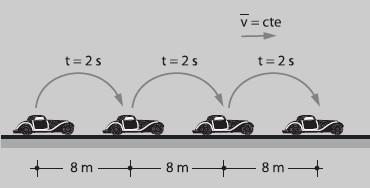
\includegraphics[scale=0.8]{images/Movimiento_rectilineo_uniforme.jpg}
 % cinematica.png: 0x0 px, 300dpi, 0.00x0.00 cm, bb=
 \caption{Ilustración del vector velocidad.}\label{mru}
\end{figure} 
 
La ilustración \ref{mru} muesta a un auto con MRU que cada 2 segundos recorre una distancia de 8 metros, esto  corresponde a 
decir que su velocidad es de $v = \frac{8m}{2s} = 4 m/s$, por lo cual despues de 6 segundos el auto habrá recorrido 24 metros.

\subsection{Problemas de mru}

\begin{enumerate}

\item Encuentre la longitud recorrida por un móvil que va a una velocidad de 1200 cm/s durante
 media hora. 

\item Un tren va a una velocidad de 200 km/h.
 ¿Qué distancia recorrerá en media hora? 

\item Calcula la velocidad expresada en unidades el SI de un camión que recorre los 90 km que
 existe entre dos ciudades 
separadas en 1 hora y 10 minutos. 

\item  Un automóvil recorre 180 m en 30 segundos. ¿Cuál es su
 velocidad? 

\item  Una partícula situada en el punto 
 (3,-4)m se mueve con velocidad constante hasta el punto (4,5)m en 12 segundos, 
determina la 
velocidad empleada

\item  Dos autos de carrera compiten entre si
 en una pista en
 línea recta cuya longitud es de 30 km. ¿Cuál será el auto 
ganador si el primero tiene una
 velocidad de 144 km/h, mientras que el segundo tiene una velocidad de 300 km/h pero

parte desde una posición de ventaja de 500 m?

\item Un coche se mueve durante 30 minutos a 40 km/h;
 después se mueve a 60 km/h durante la siguiente hora. Finalmente durante 
15 minutos
 circula a 20 km/h. ¿Qué distancia total habrá recorrido?
 
\item En el mismo instante, una motocicleta sale de la ciudad A y otra de la ciudad B, con la intención de encontrarse en el 
camino recto de 60 kilómetros que une ambas ciudades. Sabiendo que las velocidades de las motocicletas son 70km/h y 55km/h, 
calcular cuánto tardarán en encontrarse.

\item En una persecución policial, el automóvil a la fuga lleva una velocidad de 150km/h cuando
 pasa por un determinado punto 
de una carretera. Tres minutos después, el automóvil oficial que sigue al
 anterior pasa por dicho punto a una velocidad de tan 
solo 240km/h para evitar causar un accidente con los
 demás vehículos de la carretera a causa de un exceso de velocidad. Se 
supone que las velocidades indicadas
 son constantes y la carretera es recta. Calcular cuánto tardará la policía en alcanzar 
al delincuente.


\item Para recorrer dos puntos que distan entre sí 200 m, un
 móvil se desplaza con una velocidad constante de 50 m/s, si se 
duplica su velocidad para
 cubrir la misma distancia , ¿cuántos segundos utilizará?

\item  Dos autos de carrera compiten entre si
 en una pista en
 línea recta cuya longitud es de 30 km. ¿Cuál será el auto 
ganador si el primero tiene una
 velocidad de 144 km/h, mientras que el segundo tiene una velocidad de 300 km/h pero

parte desde una posición de ventaja de 500 m?

\item  La velocidad de la luz en el vacío es, 
aproximadamente, v = 300.000 km/s. ¿Cuánto tarda en llegar la luz del Sol al 
planeta Tierra si éstos 
distan unos 149,6 millones de kilómetros?


\item  Dos trenes parten de una misma
 estación; uno a 50 km/h y el otro a 72 km/h. ¿A qué distancia se encontrarán al cabo de 
media
 hora si marchan en sentido contrario? 


\item  ¿En que momento se cruzan dos 
 autos que parten de dos ciudades que distan 80 km, si sus velocidades son de 70 km/h y 90 
km/h, 
respectivamente y que van al encuentro del uno con respecto al otro?

\item  Un auto viaja con MRU y debe llegar a su destino a las
 8.00 PM. Si viajara a 140 km/h llegarııa una hora después y si 
viajara a 180 km/h llegaría
 media hora antes. ¿A qué velocidad debe el auto viajar para que llegar a la hora indicada?

\item Dos
 móviles están separados 200 km, y se mueven al encuentro llegando a cruzarse al cabo
 de 8 horas. Calcula la velocidad 
del más veloz, si la velocidad del otro es 2 km/h menos. 
\end{enumerate}
